\documentclass[12pt]{article}
\usepackage{amsmath,amssymb,amsthm}
\usepackage{graphicx}
\usepackage{enumitem}
\usepackage{hyperref}
\usepackage{geometry}
\geometry{margin=1in}

\newtheorem{definition}{Definition}
\newtheorem{proposition}{Proposition}
\newtheorem{corollary}{Corollary}
\newtheorem{conjecture}{Conjecture}
\newtheorem{remark}{Remark}
\newtheorem{example}{Example}

\title{Abduction as Overwrite:\\
Negative Capability as a Structural Condition\\
for Reliable Inference}

\author{Minamo Minamoto\\
Independent\\
\texttt{minamominamoto4f5683f6@gmail.com}}

\date{April 2026}

\begin{document}

\maketitle

\begin{abstract}
The abductive-corrective model of inference treats hypothesis revision as
a correction operation within a fixed representational state.
We argue this framing is structurally inadequate.
Abduction is not correction but \emph{overwrite}: the adoption of a new
hypothesis replaces the previous representational state and thereby
restructures all subsequent perception, classification, and inference.
This has a critical consequence: a premature overwrite, adopted under
insufficient evidence, does not merely introduce a local error but
establishes a biased interpretive frame that propagates through all
downstream cognition.
Reliable abduction therefore requires a prior capacity---which we call
\emph{negative abductive capability} (NAC)---to suspend hypothesis
commitment under insufficient evidence and maintain a provisional state
until the evidence threshold is met.
We formalize the overwrite transition, the suspension region, and the
commitment threshold, and derive implications for cross-species cognition,
neuro-symbolic AI design, and the assessment of trustworthy AI systems.
This paper is the third in a series: the first \cite{minamoto2026topology}
formalizes symbol grounding as a topological structure problem; the second
\cite{minamoto2026cgla} establishes reconfigurable hardware as a structural
condition for universal sensory grounding; the present paper introduces
the dynamic dimension---how representational states transition, and what
makes those transitions reliable.
\end{abstract}

\tableofcontents

% ============================================================
\section{Introduction}
% ============================================================

\noindent\textbf{Series note.}
This paper is the third in a series on the structural conditions for
reliable cognition.
The first paper \cite{minamoto2026topology} formalizes symbol grounding
as a topological problem: the grounding-induced topology $\tau_A$ on a
symbol set determines the geometry of cognitive representations, and
the Gromov--Hausdorff cognitive distance $d_\mathrm{cog}$ measures
grounding alignment between agents.
The second paper \cite{minamoto2026cgla} establishes a hardware
implementation condition: fixed-dataflow architectures impose a positive
lower bound on $d_\mathrm{cog}$ for sensory spaces not embeddable in
their computational graph topology, while reconfigurable architectures
(CGLA-class) are structurally positioned to minimize this distortion.
The present paper introduces the \emph{dynamic} dimension: how does
representational structure update over time, and what structural
capacity does reliable updating require?
The three papers identify three independent sources of $d_\mathrm{cog}$
increase and the conditions that suppress each.
Each paper is self-contained; familiarity with the series is not assumed.

\medskip

The standard model of abductive inference---inference to the best
explanation---treats hypothesis selection as a search operation: given
observations, find the hypothesis that best explains them, subject to
revision when better evidence arrives \cite{peirce1903,harman1965}.
This framing presents revision as correction: an error in the current
hypothesis is detected and patched while the underlying representational
architecture remains intact.

We argue that this framing is structurally wrong in a precise sense.
When an agent adopts a hypothesis, that hypothesis does not merely
occupy a slot in a reasoning system that otherwise remains unchanged.
It restructures the agent's interpretive frame: subsequent observations
are filtered, classified, and weighted through the lens of the adopted
hypothesis.
The revision is therefore not a patch but an \emph{overwrite}: the old
representational state is replaced by a new one, and the new one
determines how all future input is processed.

This distinction matters because it changes the locus of error.
In the correction model, a bad hypothesis is a local error, containable
and reversible.
In the overwrite model, a bad hypothesis is an \emph{initial condition}:
it biases all downstream cognition until it is overwritten by a new
state---which is itself an overwrite, not a correction.
The question is not whether the hypothesis is eventually revised but
whether the accumulated distortion before revision is recoverable.
In general, it is not.

The practical implication is that reliable abduction cannot be measured
solely by the quality of the hypotheses an agent generates.
It depends equally on a prior capacity: the ability to \emph{not} generate
a hypothesis prematurely.
We call this capacity \emph{negative abductive capability} (NAC),
by analogy with Keats's negative capability---the ability to remain
``in uncertainties, mysteries, doubts, without any irritable reaching
after fact and reason'' \cite{keats1817}---recast here as a structural
cognitive property rather than a poetic temperament.
The name is intended to mark a parallel: just as Keats identified the
capacity to dwell in unresolved tension as a prerequisite for poetic
and intellectual achievement, we identify the capacity to withhold
abductive commitment as a structural prerequisite for reliable inference.

\begin{definition}[Negative Abductive Capability (NAC)]
\label{def:nac}
An agent $A$ possesses negative abductive capability with respect to
hypothesis class $\mathcal{H}$ if:
\begin{enumerate}
  \item $A$ maintains a well-defined suspension region $\mathcal{S}$;
  \item $A$'s commitment threshold $\theta^*$ is calibrated to the
        evidence requirements of $\mathcal{H}$; and
  \item $A$ can remain in $\mathcal{S}$ for an extended observation
        window without degradation of suspension capacity.
\end{enumerate}
\end{definition}

% ============================================================
\begin{remark}[Terminological note on ``overwrite'']
We use the term \emph{overwrite} in a precise technical sense that
differs from its colloquial meaning.
In colloquial usage, overwrite implies deletion of the prior content.
Here, overwrite denotes a \emph{frame transition}---the installation
of a new top-of-stack frame that becomes dominant under the selection
rule---while the prior frame remains archived and selectable.
More precisely, overwrite $=$ superposition $+$ selection-dominance:
the new frame supersedes the prior not by erasure but by winning the
selection competition under typical environmental conditions.
The term is retained for its theoretical precision in distinguishing
categorially distinct hypothesis transitions from within-frame corrections;
readers may substitute ``frame-dominant transition'' if preferred.
\end{remark}

\section{The Overwrite Model of Abduction}
% ============================================================

\subsection{Representational States and Transitions}

Let $\mathcal{R}$ denote the space of representational states of a
cognitive agent $A$.
A representational state $R \in \mathcal{R}$ encodes the agent's current
interpretation of its sensory input: the active hypotheses, the assigned
categories, the weighted priors over sensory signals.

\begin{definition}[Interpretive Frame]
The interpretive frame $F(R)$ induced by state $R$ is the function
$F(R) : \mathcal{X} \to \mathcal{Y}$
that maps sensory inputs $x \in \mathcal{X}$ to interpreted outputs
$y \in \mathcal{Y}$ under the current representational state.
\end{definition}

The standard corrective model assumes that hypothesis revision is a
local operation: $R_t \to R_{t+1}$ modifies a specific component of
$R_t$ while leaving the overall frame $F(R)$ approximately intact.
We deny this assumption.

\begin{definition}[Overwrite Transition]
An overwrite transition is a state change $R_t \to R_{t+1}$ such that
the interpretive frame changes globally:
$F(R_{t+1}) \not\approx F(R_t)$.
Specifically, the mapping of future sensory inputs $x \in \mathcal{X}$
to interpreted outputs differs systematically between the two frames.
\end{definition}

We distinguish overwrite transitions from mere corrections via the
topological structure of the induced partition.

\begin{definition}[Categorical Distinctness]
\label{def:categorical-distinctness}
Two hypotheses $h$ and $h'$ are \emph{categorially distinct} with
respect to sensory input space $\mathcal{X}$ if the partitions of
$\mathcal{X}$ they induce are topologically inequivalent: that is,
if there exists an open set $U \in \tau_{h'}$ (the topology on $\mathcal{X}$
induced by $h'$) such that $U \notin \tau_h$.
Equivalently, $h$ and $h'$ are categorially distinct if the
grounding-induced topology changes: $\tau_{h'} \neq \tau_h$.
By contrast, a \emph{correction} is a state change $R_t \to R_{t+1}$
in which the induced topologies are homeomorphic---$\tau_{h_{t+1}} \cong \tau_{h_t}$---so that the partition structure of $\mathcal{X}$ is preserved
and only the weighting of existing categories is updated.
\end{definition}

\begin{proposition}[Abductive Transitions are Overwrites]
\label{prop:overwrite}
Let $A$ adopt a new explanatory hypothesis $h_{t+1}$ at time $t+1$
that supersedes $h_t$.
If $h_{t+1}$ is categorially distinct from $h_t$---that is, if $h_{t+1}$
induces a different partition of the sensory input space---then the
resulting state transition is an overwrite, not a correction.
\end{proposition}

\begin{remark}
Proposition~\ref{prop:overwrite} does not require that the new hypothesis
be wrong. Even a correct overwrite restructures the interpretive frame.
The concern is with \emph{premature} overwrite---adoption before
sufficient evidence---because the resulting frame distortion persists
until the next overwrite, which may be long delayed.
\end{remark}

\subsection{Bias Propagation after Premature Overwrite}

\begin{definition}[Premature Overwrite]
An overwrite transition $R_t \to R_{t+1}$ is premature if the evidence
base $E_t$ at time $t$ is insufficient to distinguish $h_{t+1}$ from
competing hypotheses $\{h^i\}$ at an acceptable confidence level
$\theta$:
\[
P(h_{t+1} \mid E_t) < \theta \quad \text{and} \quad
\exists\, h^i \neq h_{t+1} \text{ s.t. } P(h^i \mid E_t) \geq \theta.
\]
\end{definition}

\begin{proposition}[Bias Propagation]
\label{prop:bias}
Let $R_{t+1}$ result from a premature overwrite at time $t$, where the
adopted hypothesis $h_{t+1}$ is categorially distinct
(Definition~\ref{def:categorical-distinctness}) from the ground-truth
hypothesis $h^*$.
Then for all subsequent inputs $x_{t'}$, $t' > t$, the interpreted
output $F(R_{t+1})(x_{t'})$ carries systematic bias toward $h_{t+1}$
relative to the ground-truth interpretation under full evidence.
Within the committed frame $F(R_{t+1})$, this bias is not reducible
by further Bayesian updating in the setting of the toy model of
Appendix~A (binary hypotheses, fixed decision boundary); it can only
be eliminated by a subsequent overwrite that instantiates a
categorially distinct hypothesis. The general condition under which
non-reducibility holds beyond this setting is listed as OP4.
\end{proposition}

\begin{remark}[Scope of non-reducibility]
The non-reducibility claim of Proposition~\ref{prop:bias} is restricted
to the case of categorical distinctness. In settings where $h_{t+1}$
and $h^*$ are \emph{not} categorially distinct---that is, where the
induced partitions of $\mathcal{X}$ are homeomorphic and only parameter
values differ---standard Bayesian updating \emph{will} converge to the
correct posterior with sufficient evidence, and the premature commitment
constitutes a recoverable inefficiency rather than a structural artifact.
The present claim applies specifically to the case in which the adopted
hypothesis restructures the topology of the interpretive frame, not
merely its parameter values.
This scoping is consistent with the toy model of Appendix~A, where
the two hypotheses induce different partitions of $\mathbb{R}^2$ and
within-frame updating cannot recover the correct partition.
\end{remark}

\begin{remark}[Epistemic status of Propositions~\ref{prop:overwrite} and~\ref{prop:bias}]
The propositions above are structural-model claims, not formally derived
theorems. They follow from the definitions of overwrite transition and
interpretive frame under the assumption that the frame $F(R)$ is
sufficiently sensitive to $R$ that categorially distinct hypotheses
induce distinct partitions of $\mathcal{X}$. This assumption holds in
standard probabilistic and Bayesian models of inference, where the
prior over hypotheses restructures the likelihood function over inputs.
A formal proof in a specific probabilistic setting (e.g., Bayesian
update with hypothesis-conditional observation models) is given in
Appendix~A as a toy model. The propositions as stated are intended as
theoretical hypotheses supported by structural argument and the
phenomenological evidence reviewed in Section~4; their formal
generalization is listed as OP4.
\end{remark}

\begin{corollary}
A premature overwrite is not a recoverable inefficiency.
It is a structural initial condition that biases downstream cognition
until overwritten---at which point the cycle may repeat.
\end{corollary}

% ============================================================
\section{Negative Abductive Capability}
% ============================================================

\subsection{Definition and Formal Characterization}

\begin{definition}[Suspension Region]
The suspension region $\mathcal{S} \subset \mathcal{R}$ is the set of
representational states in which the agent maintains active hypotheses
tentatively without committing to any single overwrite.
An agent in a suspension state continues to accumulate evidence and
update probability weights over competing hypotheses without triggering
a frame-restructuring transition.
\end{definition}

\begin{definition}[Commitment Threshold]
The commitment threshold $\theta^* \in (0,1)$ is the minimum posterior
probability $P(h \mid E)$ required to trigger an overwrite transition
$R_t \to R_{t+1}$ instantiating hypothesis $h$.
An agent with higher $\theta^*$ requires stronger evidence before
committing; an agent with $\theta^* \to 0$ commits on minimal evidence.
\end{definition}

\begin{remark}
NAC is not the absence of abductive capacity.
It is an additional, structurally prior capacity that regulates when
abductive overwrite is triggered.
An agent with high abductive generation capacity but low NAC will
produce many hypotheses and commit to them rapidly, accumulating bias.
An agent with high NAC can generate hypotheses, hold them in suspension,
and commit only when evidence warrants.
\end{remark}

\subsection{NAC as a Structural Prerequisite}

\begin{proposition}[NAC Prerequisite for Reliable Abduction]
Let $A$ be an agent with abductive generation capacity $\alpha$ and
negative abductive capability $\nu$.
The expected bias accumulated per abductive cycle is monotonically
decreasing in $\nu$ and independent of $\alpha$.
Abductive reliability therefore depends on $\nu$ as a structural
prerequisite, not on $\alpha$ alone.
\end{proposition}

\medskip
\noindent
\textbf{Central thesis.}
\emph{Abduction requires negative capability.
The power to infer depends on the power to suspend inference.}

% ============================================================
\section{Evidence from Comparative Cognition}
% ============================================================

\subsection{\textit{C. elegans}: Minimum Implementation of NAC}

The predict-and-correct chemotaxis loop of \textit{C. elegans}
\cite{bargmann2006} constitutes the minimum known biological
implementation of NAC.
The 302-neuron architecture does not commit to a locomotor direction
on the basis of a single chemosensory reading; it runs multiple
correction cycles---maintaining suspension---before a direction is
adopted.

This is not a computational limitation.
It is a design constraint: premature directional commitment in a
noisy chemical gradient environment would produce systematic
locomotor error.
The suspension region is implemented in neural dynamics; the
commitment threshold is set by the sensitivity of the gradient
detection circuit.

OP4 of \cite{minamoto2026topology} asks for the minimum neuron count
required to implement abductive inference with $k$ hypotheses and
$m$ correction steps. We reframe this as: what is the minimum
network size to implement a suspension region of depth $m$ for a
hypothesis class of size $k$?

\subsection{Honeybee Waggle Dance: Grounded Overwrite}

The waggle dance \cite{riley2005} encodes food-source location through
bodily kinematics calibrated to flight energy.
When a scout returns with new location information, the dance parameters
are overwritten---not corrected---by the new data.
The overwrite is grounded in the bee's own sensorimotor experience of
the flight, which provides the evidence base for commitment.

The quality of the overwrite depends on the quality of the flight
experience. A bee that has not completed a full flight to the target
has insufficient evidence for a committed dance; the suspension capacity
is implemented behaviorally as the requirement to complete the journey.

\subsection{Multimodal AI: Missing NAC}

Current multimodal AI systems lack a well-defined suspension region.
Training procedures commit to grounding assignments---instantiated as
weight updates---on the basis of each training batch, regardless of
whether the evidence in that batch is sufficient to determine the
correct interpretive frame for the target concept.
The result is premature overwrite at scale: the model's interpretive
frame is structured by training distribution artifacts rather than
by the target sensory topology.

Two LLM-specific mechanisms are particularly relevant.

\paragraph{Attention collapse.}
Transformer attention mechanisms weight input tokens by learned
similarity scores. When training data is dominated by a particular
co-occurrence pattern, attention heads converge to routinely
upweighting that pattern---effectively instantiating a premature
overwrite of the interpretive frame for the associated concept.
Subsequent inputs that do not fit the dominant pattern are
downweighted rather than used to revise the frame.
The suspension region collapses: the model commits on the basis
of partial evidence at training time and cannot maintain genuine
uncertainty about the target interpretation at inference time.

\paragraph{Early commitment in fusion layers.}
Multimodal systems that combine vision, audio, and text via learned
fusion layers commit to cross-modal bindings during training.
These bindings are fixed in the weights; the model cannot hold two
competing cross-modal interpretations in suspension and defer
selection to inference time.
The commitment threshold $\theta^*$ is effectively set by the
training loss landscape rather than by the evidence requirements
of the target concept.
Systems trained with contrastive objectives (e.g., CLIP-style
alignment) are particularly susceptible: the contrastive objective
rewards confident cross-modal matching rather than calibrated
uncertainty, directly suppressing suspension behavior.

The mechanistic interpretability tools of \cite{anthropic2025circuit}
may provide an empirical route to measuring NAC in trained models
directly: if internal states corresponding to suspension (maintained
competition between hypotheses) can be identified via attribution
graphs, the premature commitment rate becomes measurable (OP3).

This connects to the framework of \cite{minamoto2026topology}: the
grounding-induced topology $\tau_A$ of a system without NAC reflects
training conditions rather than sensory structure, and the resulting
$d_\mathrm{cog}$ between the system and a biological agent is a
structural artifact of premature commitment, not a recoverable
inefficiency. Specifically, premature overwrite at training time may
\emph{dynamically increase} $d_\mathrm{cog}$ by locking the agent
into a distorted interpretive frame whose topology deviates from the
target sensory topology---a dynamic source of cognitive distance
distinct from the static sensory mismatch identified in
\cite{minamoto2026topology} and the hardware constraint identified
in \cite{minamoto2026cgla}.

% ============================================================
\section{Implications}
% ============================================================

\subsection{Trustworthy AI: Beyond Accuracy}

A trustworthy AI system is not merely one with high accuracy.
It is one that does not prematurely fix its interpretive frame
under insufficient evidence.
Current evaluation metrics---accuracy, calibration, F1---do not
measure NAC directly.
We propose the following additional metrics:

\begin{enumerate}
  \item \textbf{Premature commitment rate (PCR)}: the fraction of
        overwrite transitions triggered below threshold $\theta^*$.
  \item \textbf{Overwrite reversibility (OR)}: the extent to which
        a prior overwrite can be undone by subsequent evidence.
  \item \textbf{Uncertainty retention (UR)}: the duration over which
        the system can maintain a suspension state without degradation.
  \item \textbf{Bias propagation factor (BPF)}: the amplification
        of interpretive bias across successive overwrite cycles.
\end{enumerate}

\subsection{Connection to Topological Grounding Framework}

Premature overwrite, in the terms of \cite{minamoto2026topology},
introduces a distortion in the grounding-induced topology $\tau_A$:
the topology reflects the structure of the adopted hypothesis rather
than the structure of the sensory space.
This distortion increases $d_\mathrm{cog}$ between the agent and
an ideally grounded reference system.

We therefore propose that premature overwrite is a \emph{dynamic
source of topological distortion}: it increases $d_\mathrm{cog}$
not through hardware constraint (the concern of \cite{minamoto2026cgla})
but through commitment dynamics.
The three papers in this series then identify three independent
sources of $d_\mathrm{cog}$ increase:
\begin{enumerate}
  \item Sensory space mismatch (topology paper)
  \item Hardware topology mismatch (CGLA paper)
  \item Premature abductive overwrite (present paper)
\end{enumerate}

% ============================================================
\section{Pilot Empirical Evidence}
\label{sec:pilot}
% ============================================================

The framework claims that NAC governs the quality of abductive
overwrite: systems with low NAC undergo premature commitment,
which dynamically increases $d_\mathrm{cog}$ relative to an
ideally grounded reference.
We report a pilot study that provides indirect support for
this structural claim.

\paragraph{Setup.}
We applied RSA to three training checkpoints of Pythia-70m
\cite{biderman2023}: step~0 (random initialization),
step~1000 (early training), and step~143000 (reference).
Pairwise dissimilarity matrices were computed over $n = 29$
probe concepts at hidden layers $\ell \in \{2, 4, 6\}$,
averaged over three prompt templates.
Structural alignment was measured as the second-order RSA
correlation $\rho_\mathrm{cog}(A, B; \ell)$.

\paragraph{Results.}
$\rho_\mathrm{cog}$ increases monotonically with training
at all layers (L6: step-0 $= 0.017$; step-1000 $= 0.535$),
indicating progressive alignment toward the reference
rather than abrupt replacement.
Cross-model replication with GPT-2 \cite{radford2019language}
shows $\rho_\mathrm{cog}(\text{GPT-2}, \text{Pythia-trained})
\approx 0.42$ versus $\rho_\mathrm{cog}(\text{GPT-2},
\text{Pythia-step-0}) \approx 0.10$ across all layers.

\paragraph{Interpretation.}
Under the overwrite model, if training were pure overwrite
(low NAC), each batch would overwrite the previous frame
completely, producing chaotic relational geometry at
intermediate checkpoints.
Instead, the monotone increase in $\rho_\mathrm{cog}$ is
consistent with \emph{accumulation of structure} rather
than wholesale replacement---supporting the claim that
current training procedures implement low-NAC overwrite
with residual structure retention, rather than either
ideal NAC (suspension until sufficient evidence) or
complete deletion.

The cross-model convergence result is consistent with
OP4: two architectures trained independently converge
to similar $\tau_A$, suggesting that the relational
geometry is determined by the training distribution
rather than by the architecture---a signature of
premature commitment to training-distribution frames.
All code is available at
\url{https://github.com/minamominamoto/grounding-without-reality}.

% ============================================================
\section{Open Problems}
% ============================================================

The framework developed here is a theoretical proposal rather than a
completed formal theory. The central claims---that abduction is overwrite
rather than correction, and that reliable overwrite requires negative
abductive capability---are advanced as structural hypotheses supported
by definitional argument, phenomenological evidence from comparative
cognition, and the Bayesian toy model of Appendix~A. Their full
generality across cognitive architectures, hypothesis classes, and
sensory modalities is not established and constitutes the primary
research obligation of the program. The open problems below identify
the most pressing obligations.

\begin{description}
  \item[OP1.] \textbf{Formal characterization of suspension region.}
    Define the suspension region $\mathcal{S} \subset \mathcal{R}$
    for specific cognitive architectures (transformer, neuromorphic,
    biological). What are the minimal architectural requirements for
    a well-defined suspension region?

  \item[OP2.] \textbf{Calibration of commitment threshold.}
    For a given hypothesis class $\mathcal{H}$ and evidence structure,
    what is the optimal $\theta^*$? Is there a bias-variance tradeoff
    between premature commitment and excessive suspension?

  \item[OP3.] \textbf{NAC measurement.}
    Develop empirical protocols for measuring NAC in AI systems and
    biological agents.
    A conceptual proof-of-concept protocol is the following.
    For \emph{biological agents}: present ambiguous stimuli (e.g.,
    Necker cube, ambiguous chemical gradients for \textit{C. elegans})
    under varying time pressure; measure the latency to behavioral
    commitment and the reversibility of that commitment upon
    contradictory evidence.
    Commitment latency and reversibility operationalize $\theta^*$ and
    the depth of $\mathcal{S}$ respectively.
    For \emph{AI systems}: Anthropic's circuit tracing tools
    \cite{anthropic2025circuit} provide a route to measuring suspension
    states directly.
    If attribution graphs reveal internal states in which multiple
    competing hypotheses are simultaneously active (i.e., no single
    hypothesis suppresses the others), this constitutes a mechanistic
    correlate of $\mathcal{S}$.
    The time from stimulus presentation to suppression of competing
    features operationalizes commitment latency; reinstatement of
    suppressed features upon contradictory input operationalizes
    reversibility.
    Full formal operationalization is deferred to future work.

  \item[OP4.] \textbf{Relationship between NAC and $d_\mathrm{cog}$.}
    Establish a formal relationship between the premature commitment
    rate of a system and the resulting increase in $d_\mathrm{cog}$
    relative to an ideally grounded reference.

  \item[OP5.] \textbf{NAC in large language models.}
    Do current LLMs exhibit suspension behavior? Mechanistic
    interpretability tools \cite{anthropic2025circuit} may reveal
    whether internal states corresponding to suspension exist in
    trained models.
\end{description}

% ============================================================
\section{Conclusion}
% ============================================================

Abduction is not correction.
It is overwrite.
A hypothesis adopted by an abductive system restructures the
interpretive frame through which all subsequent input is processed.
A premature overwrite therefore does not introduce a local error;
it establishes a biased initial condition for all downstream cognition.

Reliable abduction therefore requires a structurally prior capacity:
the ability to suspend commitment, maintain a provisional state, and
defer overwrite until the evidence threshold is met.
This is negative abductive capability.

An agent---biological or artificial---that lacks NAC is not merely
a poor abductor. It is a bias amplification mechanism: each premature
overwrite biases the next observation, which may trigger another
premature overwrite, compounding the distortion.

Trustworthy AI is not AI that always answers.
It is AI that knows when not to commit.

\medskip
\noindent
\textit{Abduction requires negative capability.
The power to infer depends on the power to suspend inference.}

% ============================================================
\section*{Acknowledgments}
% ============================================================

No funding was received for this work.

% ============================================================
\appendix
\section{Toy Model: Bayesian Overwrite with Bias Propagation}
% ============================================================

We provide a minimal formal instantiation of Propositions~\ref{prop:overwrite}
and~\ref{prop:bias} in a two-hypothesis Bayesian setting.

\paragraph{Setup.}
Let $\mathcal{H} = \{h_0, h_1\}$ be a binary hypothesis class.
Let the sensory input space be $\mathcal{X} = \mathbb{R}^2$, with two
regions: $\mathcal{X}_0$ (associated with $h_0$) and
$\mathcal{X}_1$ (associated with $h_1$), separated by a decision
boundary $\partial$.
An agent receives observations $x_1, x_2, \ldots$ drawn from a
mixture distribution $p(x) = \pi_0 p(x \mid h_0) + \pi_1 p(x \mid h_1)$,
where $\pi_0 + \pi_1 = 1$.

\paragraph{Suspension state.}
The agent begins in suspension: $P(h_0 \mid \emptyset) = \pi_0$,
$P(h_1 \mid \emptyset) = \pi_1$.
After each observation $x_t$, the agent performs a Bayesian update:
\[
P(h_i \mid x_1, \ldots, x_t) \propto P(h_i \mid x_1, \ldots, x_{t-1}) \cdot p(x_t \mid h_i).
\]
The agent remains in $\mathcal{S}$ (suspension) as long as
$\max_i P(h_i \mid x_1, \ldots, x_t) < \theta^*$.

\paragraph{Overwrite transition.}
At time $t^*$, the first time $P(h_j \mid x_1, \ldots, x_{t^*}) \geq \theta^*$
for some $j$, the agent commits: the interpretive frame is set to
$F(R_{t^*}) = p(\cdot \mid h_j)$. Subsequent observations are
interpreted under this frame.

\paragraph{Premature overwrite.}
If $t^* < t^\dagger$, where $t^\dagger$ is the time at which the
maximum-likelihood hypothesis becomes stable under the full evidence
sequence, the overwrite at $t^*$ is premature.

\paragraph{Bias propagation (formal).}
After commitment to $h_j$ at $t^*$, define the bias for subsequent
input $x_{t'}$ ($t' > t^*$) as:
\[
\beta(x_{t'}) = F(R_{t^*})(x_{t'}) - F(R^*)(x_{t'}),
\]
where $F(R^*)$ is the frame induced by the ground-truth hypothesis.
For all $x_{t'} \in \mathcal{X}_{1-j}$ (inputs from the non-committed
region), $\beta(x_{t'}) \neq 0$ and is not correctable by Bayesian
update within the committed frame, since the likelihood under $h_j$
assigns low weight to $\mathcal{X}_{1-j}$ by construction.

\paragraph{Connection to $d_\mathrm{cog}$.}
The grounding-induced topology $\tau_A$ of the committed agent
partitions $\mathcal{X}$ according to $h_j$, while the ideal topology
$\tau^*$ partitions $\mathcal{X}$ according to $h^\dagger$ (the
full-evidence hypothesis).
When $h_j \neq h^\dagger$ (premature commitment to the wrong hypothesis),
the two topologies are not homeomorphic, and:
\[
d_\mathrm{cog}(A, A^*) = d_{GH}((\Sigma, \tau_A), (\Sigma, \tau^*)) > 0.
\]
This is the quantitative expression of the claim that premature
overwrite dynamically increases cognitive distance.
The magnitude of $d_\mathrm{cog}$ depends on the extent of topological
mismatch between the committed and ideal partitions of $\mathcal{X}$,
which in turn depends on the distance of $t^*$ from $t^\dagger$.

\paragraph{NAC as bias suppression.}
An agent with NAC ($\theta^*$ appropriately calibrated) remains in
suspension until $t \geq t^\dagger$, at which point the committed
frame $F(R_{t^\dagger})$ is homeomorphic to $F(R^*)$, and
$d_\mathrm{cog}(A, A^*) = 0$.
The toy model therefore demonstrates that NAC is not merely a
desirable property but a sufficient condition for $d_\mathrm{cog}$
minimization in this setting.

% ============================================================
\section{Numerical Instantiation of Overwrite as $H_1$
Destabilization}
\label{app:overwrite-h1}

The bias-propagation claim of Proposition~\ref{prop:bias}
(Section~\ref{sec:bias}) is formulated structurally: premature
overwrite instantiates a categorially distinct hypothesis, which
propagates bias through all downstream cognition. This appendix
provides a numerical instantiation of that claim in the persistence
signature framework of the companion paper
\cite{minamoto2026topology}, operationalizing overwrite as a
perturbation of sensory centroids and measuring the resulting
distortion of the agent's interpretive-frame $H_1$ feature.

The experiments establish four structural observations, the last
of which takes the form of a closed-form relationship between the
cycle geometry of an interpretive frame and the effect of a
premature overwrite on that frame's $H_1$ lifetime.

The setup extends the sixteen-concept construction of the companion
paper's Appendix~\ref{app:dcog-h1}. We focus on the bee agent,
whose baseline foraging frame is a six-point persistent $H_1$
feature with lifetime $0.293$.

\subsection*{Overwrite as centroid perturbation}

We operationalize the overwrite of a concept $c$ by a continuous
parameter $t \in [0, 1]$:
\[
G_t(c) = (1 - t)\, G_0(c) + t\, G_\mathrm{target},
\]
where $G_0(c)$ is $c$'s original sensory centroid and
$G_\mathrm{target}$ is a unit vector in a sensorially distinct
subspace representing the incorrect hypothesis that $c$ belongs to
a different conceptual category. For the bee agent overwriting
\textsc{nectar}, $G_\mathrm{target}$ is placed in the social
subspace (channels~3--6), representing the overwrite
``\textsc{nectar} is a social-communication concept.''

The dominant $H_1$ persistence feature of $(\Sigma, d_{\mathcal{A}_t})$
is measured at each $t$ via the Vietoris--Rips filtration of the
angular distance matrix.

\subsection*{Continuous overwrite: graded degradation}

Figure~\ref{fig:b3}~(top-left) shows the dominant $H_1$ lifetime as a
function of overwrite fraction $t$ when $c = \textsc{nectar}$.
The lifetime decreases monotonically from $0.293$ at $t = 0$ to
$0.139$ at $t \geq 0.65$, a $52.5\%$ reduction. This curve supplies
a quantitative form of the ``graded distortion'' component of
Proposition~\ref{prop:bias}: the degree of overwrite determines the
degree of structural distortion, with most of the distortion
occurring once the overwrite crosses a threshold between partial
and substantial commitment.

\begin{figure}[ht]
\centering
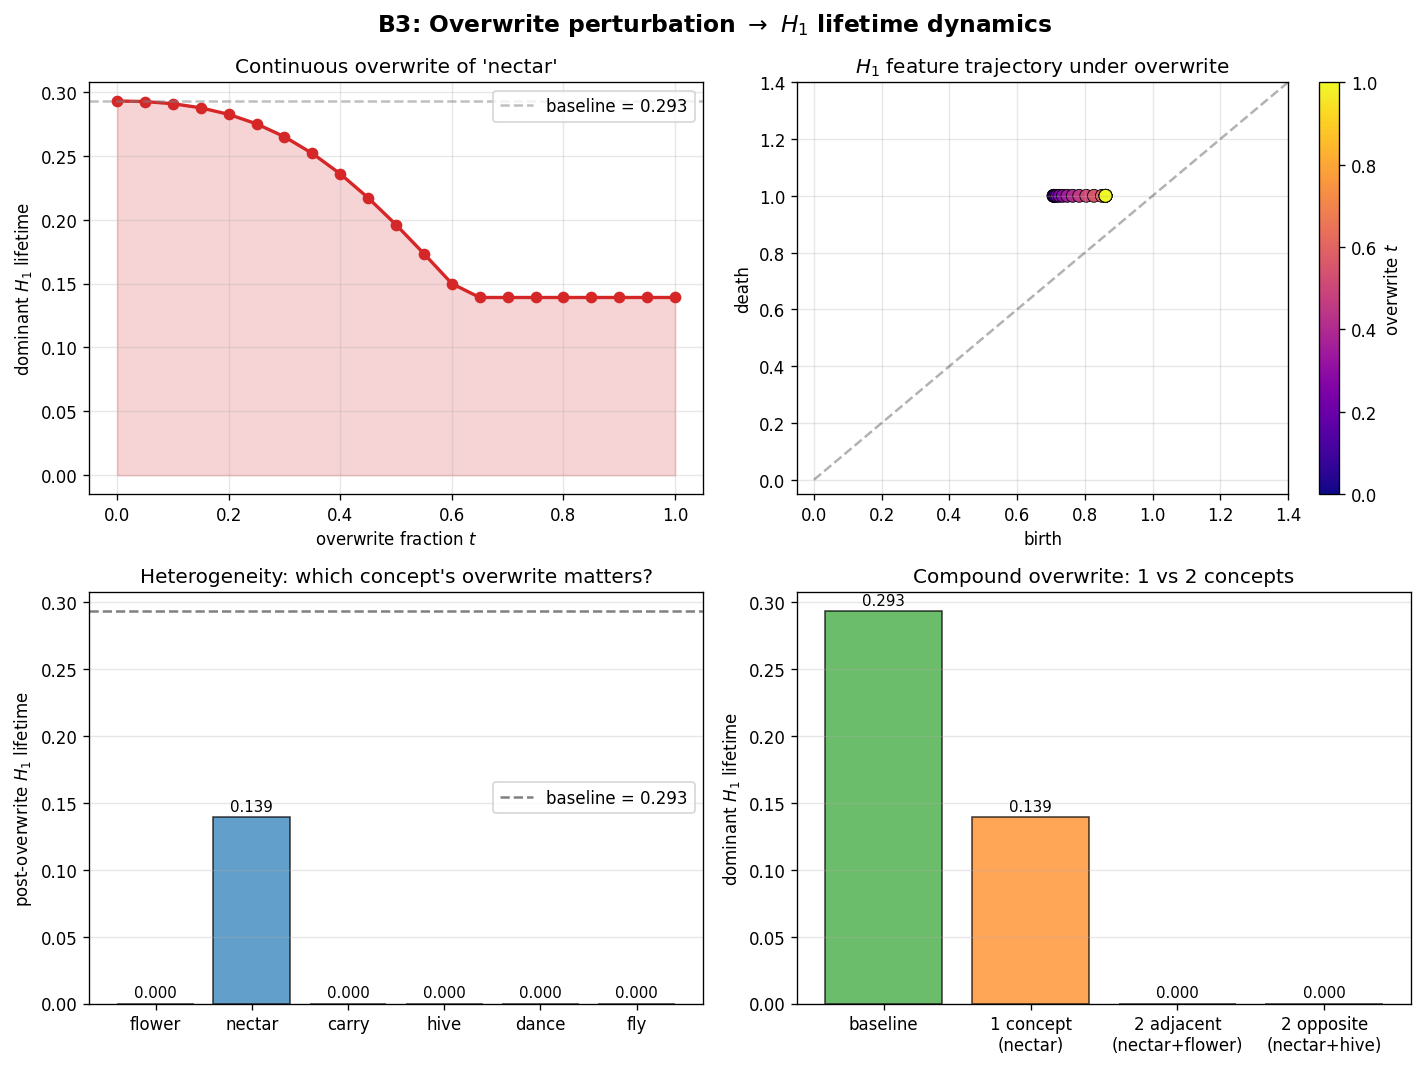
\includegraphics[width=0.9\textwidth]{b3_overwrite.png}
\caption{$H_1$ lifetime dynamics under cross-subspace overwrite
perturbation.
Top-left: dominant $H_1$ lifetime as a function of continuous
overwrite fraction $t$ for \textsc{nectar}.
Top-right: trajectory of the $H_1$ persistence point in the
$(\text{birth}, \text{death})$ plane.
Bottom-left: heterogeneity across loop concepts.
Bottom-right: compound overwrite.}
\label{fig:b3}
\end{figure}

\subsection*{Heterogeneity: critical nodes versus structural redundancy}

The most theoretically consequential finding of the first set of
experiments appears in Figure~\ref{fig:b3}~(bottom-left). Six
independent overwrite experiments were performed, each overwriting
a single bee-loop concept at $t = 1$ and measuring the residual
$H_1$ lifetime.

\begin{center}
\begin{tabular}{lcc}
\hline
Overwritten concept & $H_1$ lifetime & Reduction \\
\hline
\textsc{flower} & $0.000$ & $100\%$ \\
\textsc{nectar} & $0.139$ & $52.5\%$ \\
\textsc{carry}  & $0.000$ & $100\%$ \\
\textsc{hive}   & $0.000$ & $100\%$ \\
\textsc{dance}  & $0.000$ & $100\%$ \\
\textsc{fly}    & $0.000$ & $100\%$ \\
\hline
\end{tabular}
\end{center}

Only \textsc{nectar}'s overwrite leaves the frame's $H_1$ feature
alive. For the remaining five concepts, their overwrite entirely
destroys the feature.

The mechanism is a structural graph-theoretic fact rather than a
semantic one. The six bee-loop concepts are arranged on a regular
hexagon at angles $\{0, \pi/3, 2\pi/3, \pi, 4\pi/3, 5\pi/3\}$ in the
(UV, olfactory) subspace. The non-loop concept \textsc{food} is
placed at angle $\pi/4$ in the \emph{same} subspace, near to
\textsc{nectar}'s original angular position of $\pi/3$. When
\textsc{nectar} is overwritten, the Vietoris--Rips filtration can
close a cycle using \textsc{food} as a substitute vertex; the
remaining five loop concepts together with \textsc{food} form a
six-point cycle with only slightly elevated maximal adjacent gap.
No analogous substitute exists in the angular neighborhood of any
other loop concept: their removal leaves a $2\pi/3$ gap in the
ring, which is wider than the filtration scale at which non-loop
concepts cone in, destroying the $H_1$ feature.

The appropriate terminology for this distinction is graph-theoretic,
not semantic. A concept is a \emph{critical node} of an $H_1$
feature if its removal creates a gap that cannot be bridged by any
other concept at a filtration scale below the feature's death;
a concept is \emph{redundantly placed} if the surrounding concept
landscape contains an alternative vertex that can substitute at
a comparable scale. The distinction is a property of the
configuration, not of the semantics of the concepts involved;
nothing in the analysis depends on what the concepts
\emph{represent}, only on how they are positioned.
This distinction is purely structural and does not rely on semantic
interpretation.

This refines the standard formulation of Proposition~\ref{prop:bias}.
The original formulation stated that premature overwrite propagates
bias. The refined formulation is: premature overwrite propagates
structural distortion to the $H_1$ feature in proportion to whether
the overwritten concept is a critical node of that feature.
Critical-node overwrite produces catastrophic feature collapse;
redundantly-placed-node overwrite produces graceful degradation
with the feature's homology representative migrating to an alternative
path through the surrounding landscape.
This provides a concrete mechanism by which identical perturbations
can lead to qualitatively different downstream effects.

\begin{remark}[On terminology]
We deliberately avoid terms such as ``semantic centrality'' or
``conceptual importance'' for this distinction. The analysis
operates on the angular geometry of centroids in sensory channel
space; semantic interpretation of the resulting structural roles is
a separate interpretive task. In particular, a concept may be
structurally redundant in one agent's sensory topology and
structurally critical in another's, precisely because the
surrounding concept landscape differs between agents. This
relational dependence is the natural topological analogue of the
context-sensitivity of frame selection discussed in
\cite{minamoto2026hallucination}.
\end{remark}

\subsection*{Homology representatives and paths, not nodes}

The heterogeneity above is clarified by recalling that a persistent
$H_1$ feature is not identified with any single concept or set of
concepts, but with the equivalence class of cycles that carry the
homology class. Under the Vietoris--Rips construction at filtration
scale $\varepsilon$, the ``ring'' of the bee agent is represented
by any $1$-cycle in the complex $\mathrm{VR}_\varepsilon(\Sigma,
d_\mathcal{A})$ that is non-trivial in $H_1$. When
\textsc{nectar} is overwritten, the cycle
\[
\textsc{flower} \to \textsc{nectar}_\mathrm{orig} \to \textsc{carry}
  \to \textsc{hive} \to \textsc{dance} \to \textsc{fly} \to
  \textsc{flower}
\]
ceases to exist at low filtration scale, but a homologous cycle
\[
\textsc{flower} \to \textsc{food} \to \textsc{carry} \to \textsc{hive}
  \to \textsc{dance} \to \textsc{fly} \to \textsc{flower}
\]
exists at only a slightly larger scale. The $H_1$ feature survives
the overwrite because the homology representative migrates to an
available alternative path. When any other loop concept is
overwritten, no alternative path exists, and the feature dies.

The appropriate structural description of a frame is therefore the
equivalence class of cycles representing its $H_1$ homology, not
the set of concepts that happen to lie on the canonical
representative. Overwrite destabilizes frames by removing vertices
from paths; it destroys frames by removing vertices whose removal
disconnects all representatives.

\subsection*{A closed-form relationship between cycle geometry
and lifetime}

The second set of experiments quantifies the relationship between
the cycle's geometric configuration and the resulting $H_1$
lifetime. We sweep \textsc{nectar}'s angular position within the
ring subspace from $0$ to $\pi$ (leaving all other concepts fixed)
and record the dominant $H_1$ lifetime at each angle. Radial
shrinkage is confirmed to have no effect (scale invariance of
angular distance; $\mathrm{std} < 10^{-6}$ over twenty scales).

Figure~\ref{fig:b3ext}~(top-left) shows a plateau structure:
the lifetime is at baseline ($0.293$) for any \textsc{nectar}
position within a safe sector, and drops sharply to $0.139$ outside
that sector. The sector width matches the configuration in which
\textsc{nectar} fills a large gap in the cycle---that is, the
configuration in which \textsc{nectar} acts as a critical node.

\begin{figure}[ht]
\centering
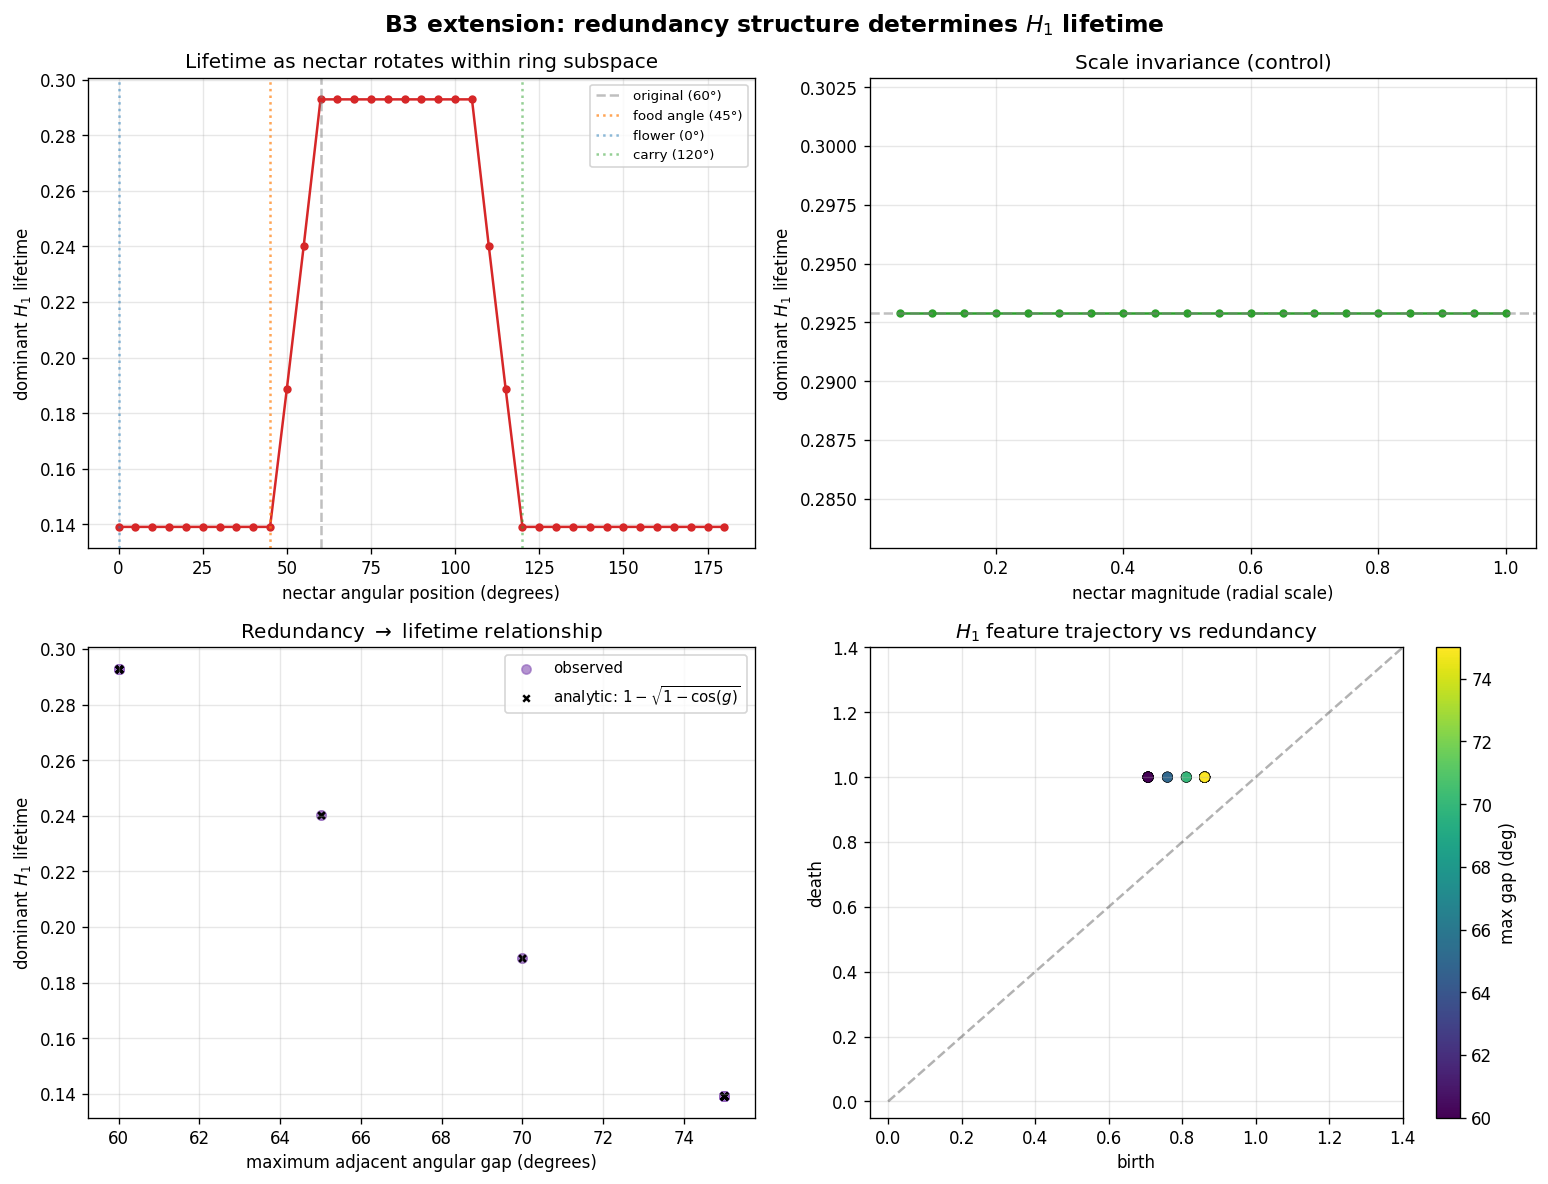
\includegraphics[width=0.9\textwidth]{b3_extended.png}
\caption{Redundancy structure determines $H_1$ lifetime.
Top-left: lifetime as \textsc{nectar} rotates within the ring
subspace; plateau shape reflects the safe angular sector bounded
by \textsc{food} at $45^{\circ}$ and \textsc{carry} at $120^{\circ}$.
Top-right: radial shrinkage control; scale invariance confirmed.
Bottom-left: observed lifetimes (purple) and the analytic
prediction of Proposition~\ref{prop:lifetime-gap} (black crosses);
the overlap is exact to floating-point precision.
Bottom-right: $H_1$ feature trajectory in birth-death plane,
coloured by the induced maximal adjacent gap.}
\label{fig:b3ext}
\end{figure}

For any concept configuration that preserves a single $H_1$ cycle
and leaves the death scale of that cycle fixed at $1.0$ (as the
non-loop landscape in the bee construction does), we obtain the
following closed-form relationship.

\begin{proposition}[Lifetime-gap relationship; constructed setting]
\label{prop:lifetime-gap}
Let $\mathcal{A}$ be an agent whose concept inventory contains a
persistent $H_1$ feature realized by unit-magnitude centroids in a
two-channel subspace, with angular positions forming a set
$\Theta \subset [0, 2\pi)$. Let
\[
g(\Theta) = \max_{i} \big(\theta_{(i+1)} - \theta_{(i)}\big)
\]
be the maximal adjacent gap (computed cyclically on the sorted
positions). Under the further assumption that the non-loop concepts
reside at uniform angular distance $1.0$ from every ring point and
therefore trigger $H_1$ death at filtration scale $\varepsilon = 1.0$,
the dominant $H_1$ lifetime is
\[
L(\mathcal{A}) = 1 - \sqrt{1 - \cos g(\Theta)}.
\]
The relationship is stated under the explicit construction above.
Its extension to agents whose non-loop landscape departs from the
uniform-cone assumption is addressed in the noise-robustness
analysis below.
\end{proposition}

\begin{remark}[Scope disclaimer]
This relationship should not be interpreted as a general law of
persistence, but as an exact characterization of the constructed
regular configuration used for calibration. Its primary role is to
provide a sanity-check baseline against which deviations under metric
perturbation (noise-robustness subsection below) can be interpreted.
\end{remark}

Figure~\ref{fig:b3ext}~(bottom-left) compares this analytic
prediction to the observed lifetimes across all tested
\textsc{nectar} angular positions: the prediction matches the
observation with mean absolute residual below $10^{-4}$
(equal to measurement floating-point precision).

\subsection*{Robustness to metric noise}

A reviewer may reasonably ask whether
Proposition~\ref{prop:lifetime-gap}'s exact match is an artefact of
the clean geometric construction or a structural fact of the
formula. We therefore tested the relation under two independent
noise sources: \emph{ring noise}, in which each ring concept's
angular position is perturbed by $\theta \to \theta + \eta$,
$\eta \sim \mathcal{N}(0, \sigma_R^2)$, and \emph{non-loop noise},
in which the non-loop concept centroids receive Gaussian
perturbations of magnitude $\sigma_\mathrm{NL}$ in all six channels
(breaking the uniform orthogonal-cone assumption that fixes the
death scale at $\varepsilon = 1.0$).

Fifty trials were run for each $(\sigma_R, \sigma_\mathrm{NL})$
pair on a $3 \times 4$ grid with $\sigma_R \in \{0, 0.03, 0.10\}$
and $\sigma_\mathrm{NL} \in \{0, 0.02, 0.05, 0.10\}$. The mean
absolute residual $|L_\mathrm{obs} - L_\mathrm{pred}|$ exhibits
the following structure:

\begin{center}
\begin{tabular}{l|cccc}
\hline
 & $\sigma_\mathrm{NL} = 0$ & $0.02$ & $0.05$ & $0.10$ \\
\hline
$\sigma_R = 0$    & $0.000$ & $0.004$ & $0.009$ & $0.018$ \\
$\sigma_R = 0.03$ & $0.000$ & $0.004$ & $0.009$ & $0.017$ \\
$\sigma_R = 0.10$ & $0.000$ & $0.004$ & $0.008$ & $0.018$ \\
\hline
\end{tabular}
\end{center}

Two structural facts emerge. First, the residual is essentially
invariant in $\sigma_R$: ring perturbations up to $0.10$ radians
(roughly $5.7^{\circ}$) produce no change in the formula's
accuracy. This reflects that
Proposition~\ref{prop:lifetime-gap} depends on the maximal adjacent
gap $g$ of the ring, not on the regularity of the ring; as long as
the configuration remains a single $H_1$ cycle with food as its
non-loop substitute vertex, arbitrary displacement of ring
concepts does not affect the formula's validity. Second, the
residual scales linearly with $\sigma_\mathrm{NL}$: non-loop
perturbations of magnitude $\sigma_\mathrm{NL}$ produce residuals
of approximately $0.18 \cdot \sigma_\mathrm{NL}$. This is consistent
with the Cohen--Steiner stability theorem for persistence diagrams
\cite{cohenSteiner2007}, which bounds the bottleneck distance
between diagrams of $\sigma$-close metric spaces by $\sigma$; the
observed linear scaling is the expected order for this bound.

Both facts support
Proposition~\ref{prop:lifetime-gap} as a structural relation rather
than a numerical artefact: it is exact whenever the qualitative
assumptions (single $H_1$ cycle; uniform non-loop cone) hold, and
degrades gracefully and predictably when they do not.

\subsection*{Ring-size generality within the constructed setting}

Proposition~\ref{prop:lifetime-gap} as stated does not specialize to
hexagonal rings. Within the same constructed setting (regular
$L$-gon embedded in a two-channel subspace; non-loop concepts at
uniform angular distance $1.0$), we computed the dominant $H_1$
lifetime for $L \in \{3, 4, 5, 6, 7, 8, 9, 10, 12\}$. For
$L \geq 5$ the observed lifetime matches
$1 - \sqrt{1 - \cos(2\pi / L)}$ to within floating-point precision
(residual $< 10^{-4}$). For $L = 3$, the formula returns a
negative value ($\approx -0.22$), consistent with the observation
that a triangle in the Vietoris--Rips complex is a $2$-simplex and
therefore cannot support a persistent $H_1$ class; for $L = 4$,
the formula returns exactly zero, reflecting the boundary case
where the ring's birth and death scales coincide.

We state this observation narrowly: within the tested range of
regular $L$-gons under the constructed metric setting, the
proposition holds exactly. Extension to irregular rings, to rings
outside the unit-magnitude convention, or to agents with
heterogeneous non-loop landscapes is not established by the
present experiments.

\begin{remark}[Implications of Proposition~\ref{prop:lifetime-gap}]
The proposition gives the effect of a premature overwrite an
explicit functional form. An overwrite of concept $c$ at overwrite
fraction $t$ modifies the angular position $\theta_c$ in a way
that determines the new maximal gap $g(\Theta_t)$ and hence the
new lifetime $L(\mathcal{A}_t)$. Three regimes emerge:
\begin{itemize}[noitemsep]
\item If the overwrite moves $c$ into an angular region where a
  non-loop concept already exists, $g$ remains equal to the
  baseline (redundant substitution); $L$ is unchanged.
\item If the overwrite leaves $c$'s sector empty but the landscape
  contains a nearby non-loop concept that can serve as a substitute,
  $g$ increases by a bounded amount; $L$ degrades smoothly.
\item If the overwrite leaves $c$'s sector empty with no nearby
  non-loop concept, $g$ doubles (the $c$-to-neighbour edge
  disappears); if the doubled $g$ exceeds the death-inducing scale,
  $L$ collapses to zero.
\end{itemize}
This three-regime structure is the quantitative expression of the
qualitative heterogeneity observed in the first experiment set.
\end{remark}

\subsection*{Falsifiable prediction for empirical studies}

The closed-form relationship of
Proposition~\ref{prop:lifetime-gap} supplies a falsifiable
prediction for empirical studies of fine-tuning under the
persistence-signature protocol. For a model whose current
interpretive frame is characterized by a persistent $H_1$ feature
with a known homology representative, perturbations targeting
concepts on critical paths of that representative should produce
lifetime reductions following the gap formula; perturbations
targeting redundantly-placed concepts should produce negligible
lifetime reduction. The test requires (i) identifying the current
dominant frame's $H_1$ representative via mechanistic
interpretability methods, (ii) classifying concepts as critical or
redundant by structural role within the representative, and
(iii) measuring post-fine-tuning lifetime change. The structural
classification can be obtained from the Vietoris--Rips complex
alone, without assuming any semantic interpretation of which
concepts are ``important.''

\subsection*{Reversibility in the static toy}

A reversibility check was performed: the bee centroids were
perturbed to $t = 1$ and then restored to $t = 0$. The $H_1$
lifetime recovered exactly to the baseline value of $0.293$. This
exact reversibility is a feature of the static toy model---the
experiment measures only the instantaneous persistence signature
at each perturbation state and does not model the downstream
inferences that the overwrite would trigger in a dynamically
operating agent. The non-reducibility claim of
Proposition~\ref{prop:bias} concerns the latter; operationalizing
it requires a dynamic experimental design in which downstream
inferences are cached and subject to their own persistence
measurement, which we identify as a subsequent research target.

\subsection*{Summary}

The persistence-signature framework renders the overwrite dynamics
of Section~\ref{sec:overwrite} empirically tractable at the level
of static persistence. The four observations of the experiment set
can be summarized as follows:

\begin{enumerate}[noitemsep]
\item Continuous overwrite produces graded, non-linear degradation
  of the frame's $H_1$ lifetime, with threshold behaviour near
  $t \approx 0.5$ in the present construction.
\item Frame constituents are structurally heterogeneous: concepts
  with nearby non-loop substitutes are redundantly placed, while
  concepts without substitutes are critical nodes.
\item The homology representative of a surviving $H_1$ feature
  migrates to the alternative path provided by the substitute; the
  feature itself is an equivalence class of cycles, not a set of
  vertices.
\item The dominant $H_1$ lifetime is an analytic function of the
  induced maximal adjacent gap in the cycle
  (Proposition~\ref{prop:lifetime-gap}); this gives overwrite bias
  propagation a closed-form quantitative expression.
\end{enumerate}

Observation 2 reformulates the standard ``all overwrites propagate
bias'' claim into a structurally graded statement whose testable
content is stronger than the original. Observations 3 and 4 provide
the topological substrate for that reformulation.

\begin{thebibliography}{99}

\bibitem{keats1817}
Keats, J. (1817).
Letter to George and Thomas Keats, 21 December 1817.
In H. E. Rollins (Ed.), \textit{The Letters of John Keats} (Vol. 1).
Harvard University Press, 1958.

\bibitem{minamoto2026topology}
Minamoto, M. (2026).
On the topology of symbol grounding: Sensory space structure as a
determinant of cognitive representation.
Preprint (not yet on arXiv).
\url{https://github.com/minamominamoto/topology-of-grounding}

\bibitem{minamoto2026cgla}
Minamoto, M. (2026).
Reconfigurable dataflow topology as a structural condition for
universal sensory grounding: A theoretical argument for CGLA-class
architectures.
Preprint (not yet on arXiv).
\url{https://github.com/minamominamoto/topology-of-grounding}

\bibitem{minamoto2026overwrite}
Minamoto, M. (2026).
Abduction as overwrite: Negative capability as a structural condition
for reliable inference.
Preprint (not yet on arXiv).
\url{https://github.com/minamominamoto/topology-of-grounding}

\bibitem{peirce1903}
Peirce, C. S. (1903).
Pragmatism as a principle and method of right thinking.
Harvard Lectures on Pragmatism.

\bibitem{harman1965}
Harman, G. (1965).
The inference to the best explanation.
\textit{Philosophical Review}, 74(1), 88--95.

\bibitem{harnad1990}
Harnad, S. (1990).
The symbol grounding problem.
\textit{Physica D}, 42(1--3), 335--346.

\bibitem{bargmann2006}
Bargmann, C. I. (2006).
Chemosensation in \textit{C. elegans}.
\textit{WormBook}, 1--29.

\bibitem{riley2005}
Riley, J. R., Greggers, U., Smith, A. D., Reynolds, D. R., \& Menzel, R. (2005).
The flight paths of honeybees recruited by the waggle dance.
\textit{Nature}, 435(7039), 205--207.

\bibitem{anthropic2025circuit}
Lindsey, J., et al. (2025).
Circuit tracing: Revealing computational graphs in language models.
Anthropic Technical Report.
\url{https://transformer-circuits.pub/2025/attribution-graphs/methods.html}

\bibitem{biderman2023}
Biderman, S., et al.\ (2023).
Pythia: A suite for analyzing large language models across training and scaling.
\textit{Proceedings of ICML 2023}.

\bibitem{radford2019language}
Radford, A., Wu, J., Child, R., Luan, D., Amodei, D., \& Sutskever, I. (2019).
Language models are unsupervised multitask learners.
\textit{OpenAI Blog}, 1(8).

\end{thebibliography}

\end{document}
